% Chapter 5

\chapter{Quantum Classifiers And Decision Boundaries} % Main chapter title

\label{chapter:quantum_classifiers_decision_boundaries}
%----------------------------------------------------------------------------------------
To analyse the expressiveness, accuracy and the impact of small gate changes for quantum classifier circuits in comparison to a classical Multi-layer Perceptron classifier (sklearn neural network \href{https://scikit-learn.org/stable/modules/generated/sklearn.neural_network.MLPClassifier.html}{\code{MLPClassifier}}), contour plots are used to visualize the decision boundaries. A quantum classifier is defined as follows by Lloyd et al.\cite{Quantum_embeddings_for_machine_learning_2020}: \textit{Let $\ket{x}$ be an embedding of a data input $x \in X$. A quantum classifier is a classifier where $f(x)$ is an expectation $\bra{x}M\ket{x}$ of a quantum measurement of the observable $M$.}
The classifier which receives the measured output of the quantum circuit (see \ref{fig:code_numpy_sign}) is defined as follows\cite{Quantum_embeddings_for_machine_learning_2020}:
\hfill \break

$f : X \rightarrow\mathbb{R}$. The quantum classifier assigns a binary label to $x$ according to the threshold rule:

\begin{equation}
    \centering
    \begin{split}
    y =
        \left\{\begin{matrix}
            -1\ if\ f(x) < \tau ,\\
            1\ if\ f(x) \geq \tau
        \end{matrix}\right.
    \end{split}
    \label{equation:classifier_definition}
\end{equation}

with $\tau\in\mathbb{R}$ and if no other information is provided, $\tau$ is assumed to be zero.\\
\hfill \break
\begin{figure}[h!]
    \centering
    \begin{minted}{python}
# Compute predictions on train and validation set
predictions_train = [np.sign(quantum_classifier(var, f)) for f in x_train]
predictions_val = [np.sign(quantum_classifier(var, f)) for f in x_test]
    \end{minted}
    \caption{Classifier uses \code{np.sign} (see \href{https://numpy.org/doc/stable/reference/generated/numpy.sign.html}{\code{numpy.sign()}}) function to assign label after classification}
    \label{fig:code_numpy_sign}
\end{figure}

Lloyd et al.\cite{Quantum_embeddings_for_machine_learning_2020} further states that quantum binary classification is defined as: \textit{For a given embedding $\Phi$, quantum binary classification is the problem of assigning $\ket{x}$ to one
of two "data-ensembles" of quantum feature states, $\varrho = \frac{1}{M_a} \sum_{a} \ket{a} \bra{a} $ or $ \sigma = \frac{1}{M_b} \sum_{b} \ket{b} \bra{b} $, where $\varrho$ and $\sigma$ are mixed states that describe the process of selecting an embedded data point $\ket{a}$, $\ket{b}$ with uniform probability from a training set.}
\hfill \break

\clearpage
The following experiments in subsections \ref{subsection:single_qubit_circuits}, \ref{subsection:two_qubit_circuits} and \ref{subsection:two_qubit_circuits_3layers} show three different artificial problems consisting of linearly separable ($make\_classfication$), circle shaped ($make\_circles$) and moon shaped data ($make\_moons$), ordered from easier to more difficult. All data sets have only two classes (binary) and are limited to $100$ data points. The data given to the quantum classifiers has been scaled to $[-1,1]$ except for the "Two qubit circuits with 3 Layers" in subsection \ref{subsection:two_qubit_circuits_3layers} where the data has been scaled to $[-\frac{\pi}{2},\frac{\pi}{2}]$.

Data was further divided into $75\%$ being used for training and $25\%$ for testing. The \href{https://www.pennylane.ai}{Pennylane.ai} framework has been used with the \href{https://pennylane.readthedocs.io/en/stable/code/api/pennylane.devices.default_qubit.html#module-pennylane.devices.default_qubit}{\code{default.qubit}} simulator. Optimization is done in a classical way with the \href{https://pennylane.readthedocs.io/en/stable/code/api/pennylane.NesterovMomentumOptimizer.html}{\code{NesterovMomentumOptimizer}} optimizer. For each iteration step, the optimizer updates the weights and gives the new values again to the quantum model circuit. The schematic setup for the quantum circuit and classical parts is identical as seen in figure \ref{fig:schematic_view_classical_and_quantum_circuit}. 

\hfill \break

\begin{figure}[h!]
    \centering
    \begin{subfigure}{0.75\textwidth}
        \begin{minted}{python}
MLPClassifier(random_state=1, max_iter=max_iterations, 
        solver="sgd", nesterovs_momentum=True)
        \end{minted}
        \caption{Python code: \code{MLPClassifier} configuration for single and 2 qubit classifier circuits (see \ref{subsection:single_qubit_circuits} and \ref{subsection:two_qubit_circuits})}
        \label{fig:code_MLPClassifier_configuration}
    \end{subfigure}
    \\[3ex]
    \begin{subfigure}{0.66\textwidth}
        \begin{minted}{python}
MLPClassifier(random_state=1, 
        hidden_layer_sizes=(100,100,100), 
        max_iter=max_iterations, solver="sgd", 
        nesterovs_momentum=True),
        \end{minted}
        \caption{Python code: \code{MLPClassifier} configuration for 2 qubit classifier circuits with 3 layers (see \ref{subsection:two_qubit_circuits_3layers})}
        \label{fig:code_MLPClassifier_configuration_3hiddenlayers}
    \end{subfigure}
    \caption{\code{MLPClassifier} configurations}
    \label{fig:MLPClassifier_configurations}
\end{figure}

All quantum circuits in subsections \ref{subsection:single_qubit_circuits}, \ref{subsection:two_qubit_circuits} and \ref{subsection:two_qubit_circuits_3layers} are finally measured in the $Z$ axis (\href{https://pennylane.readthedocs.io/en/stable/code/api/pennylane.PauliZ.html}{PauliZ}) for qubit $q_0$. 

\begin{figure}[h!]
    \centering
    \begin{minted}{python}
                @qml.qnode(dev)
                def circuit(weights, data):
                    ...
                    return qml.expval(qml.PauliZ(0))
    \end{minted}
    \caption{Python code: Circuit measurement of $Z$ axis for qubit $q_0$}
    \label{fig:code_quantum_classifiers_measurement}
\end{figure}

\clearpage
\subsection{Single Qubit Circuits}
\label{subsection:single_qubit_circuits}

In this subsection, two single qubit quantum classifiers with angle embedding for the features $\mathrm{x_0}$, $\mathrm{x_1}$ and a total count of six weights ($\mathrm{w_0}$, …, $\mathrm{w_5}$) have been trained. For comparison, there is also a Multi-layer Perceptron classifier in the plots with the same iteration count as the quantum classifiers. Figure \ref{fig:SingleQubitClassifiers_50Iterations} has a iteration count of 50, figure \ref{fig:SingleQubitClassifiers_200Iterations} shows 200 iterations and the last figure \ref{fig:SingleQubitClassifiers_400Iterations} shows the classifiers after 400 iterations. The single qubit quantum classifier circuits can be seen in figures \ref{fig:single_qubit_circuit_1} and \ref{fig:single_qubit_circuit_2}.\\
\\

\begin{figure}[h!]
    \centering

    \begin{subfigure}{1.0\textwidth}
        \centering
        \scalebox{0.66}{
            \Qcircuit @C=1.0em @R=0.2em @!R { \\
            	 	\nghost{ {q}_{0} :  } & \lstick{ {q}_{0} :  } & \gate{\mathrm{R_Y}\,(\mathrm{\color{magenta}x_0})} & \gate{\mathrm{R_Z}\,(\mathrm{\color{gray}w_0})} & \gate{\mathrm{R_Y}\,(\mathrm{\color{gray}w_1})} & \gate{\mathrm{R_Z}\,(\mathrm{\color{gray}w_2})} & \gate{\mathrm{R_Y}\,(\mathrm{\color{magenta}x_1})} & \gate{\mathrm{R_Z}\,(\mathrm{\color{gray}w_3})} & \gate{\mathrm{R_Y}\,(\mathrm{\color{gray}w_4})} & \gate{\mathrm{R_Z}\,(\mathrm{\color{gray}w_5})} & \qw & \qw\\ 
            \\ }
        }
        \caption{\textbf{Quantum Circuit classifier 1} with only $\mathrm{RY}$ and $\mathrm{RZ}$ gates using 6 weights ($\mathrm{w_0}$, …, $\mathrm{w_5}$) and two input features $\mathrm{x_0}$, $\mathrm{x_1}$ }
        \label{fig:single_qubit_circuit_1}
    \end{subfigure}
    \\[2ex]
    \begin{subfigure}{1.0\textwidth}
        \centering
        \scalebox{0.66}{
            \Qcircuit @C=1.0em @R=0.2em @!R { \\
            	 	\nghost{ {q}_{0} :  } & \lstick{ {q}_{0} :  } & \gate{\mathrm{R_Y}\,(\mathrm{\color{magenta}x_0})} & \gate{\mathrm{R_Z}\,(\mathrm{\color{gray}w_0})} & \gate{\mathrm{R_Y}\,(\mathrm{\color{gray}w_1})} & \gate{\mathrm{R_Z}\,(\mathrm{\color{gray}w_2})} & \gate{\mathrm{R_X}\,(\mathrm{\color{magenta}x_1})} & \gate{\mathrm{R_Z}\,(\mathrm{\color{gray}w_3})} & \gate{\mathrm{R_Y}\,(\mathrm{\color{gray}w_4})} & \gate{\mathrm{R_Z}\,(\mathrm{\color{gray}w_5})} & \qw & \qw\\ 
            \\ }
        }
        \caption{\textbf{Quantum Circuit classifier 2} with $\mathrm{RY}$, $\mathrm{RZ}$ gates and a $\mathrm{RX}$ gate using also 6 weights ($\mathrm{w_0}$, …, $\mathrm{w_5}$) and two input features $\mathrm{x_0}$, $\mathrm{x_1}$ }
        \label{fig:single_qubit_circuit_2}
    \end{subfigure}
    
    \caption{Single qubit quantum circuits referring to \textbf{Quantum Circuit classifier 1} and \textbf{Quantum Circuit classifier 2} in figures \ref{fig:SingleQubitClassifiers_50Iterations}, \ref{fig:SingleQubitClassifiers_200Iterations} and \ref{fig:SingleQubitClassifiers_400Iterations}.}
    \label{fig:single_qubit_circuits}
\end{figure}

% Contour and box plots
\begin{figure}[h!]
    \centering
    \caption{Decision boundary and accuracy comparison between Multi-layer Perceptron classifier, Quantum Circuit classifier 1 and Quantum Circuit classifier 2.\\\textit{Row 1}: Linearly separable data / \textit{Row 2}: Circle shaped data / \textit{Row 3}: Moon shaped data}
    \begin{subfigure}{1.0\textwidth}
        \centering
        \scalebox{0.27}{
            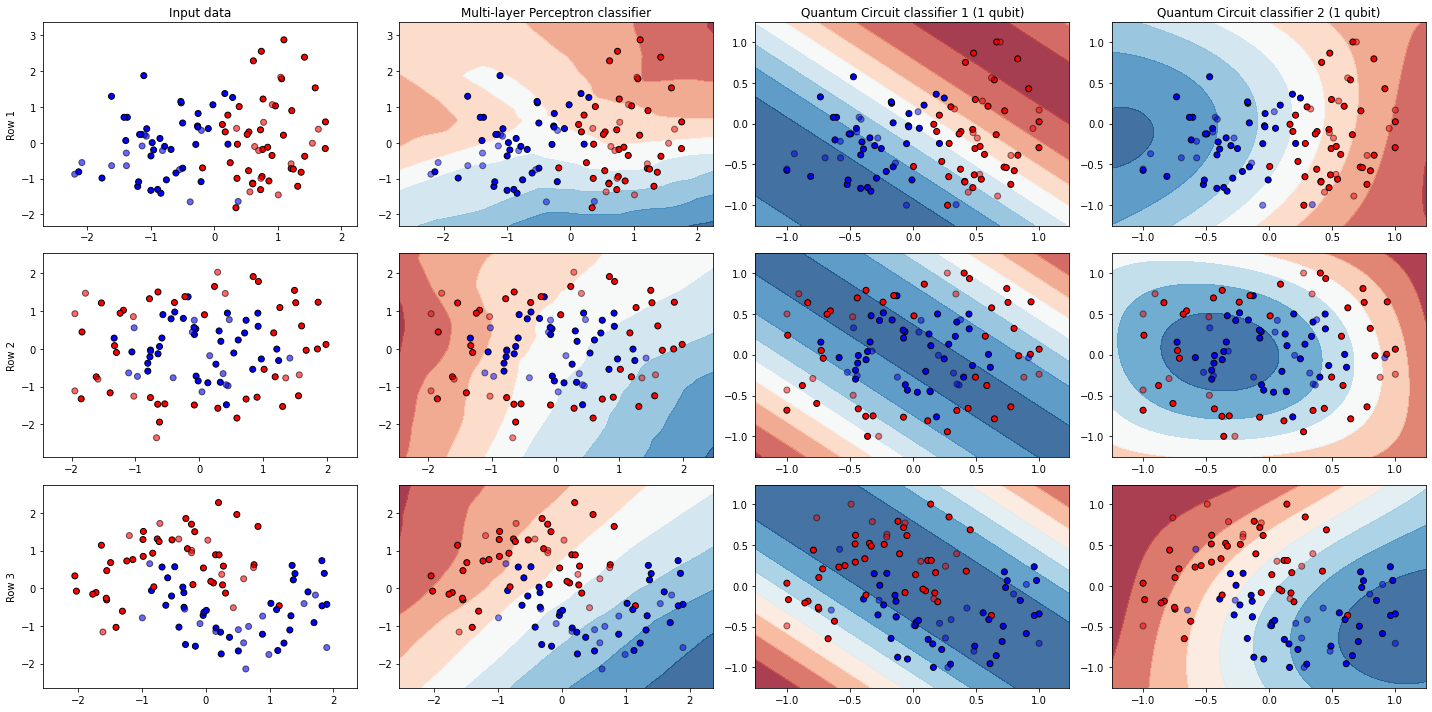
\includegraphics{Appendices/chapter_5/decision_boundary_1qubit_50-iter_01.png}
        }
        \caption{Decision boundary plot: \textbf{50 iterations} for all classifiers using \textbf{single qubit quantum circuits}.}
        \label{fig:SingleQubitClassifiers_50Iterations}
    \end{subfigure}
    \\[1ex]
    \begin{subfigure}{1.0\textwidth}
        \centering
        \begin{subfigure}{1.0\textwidth}
            \centering
            \scalebox{0.45}{
                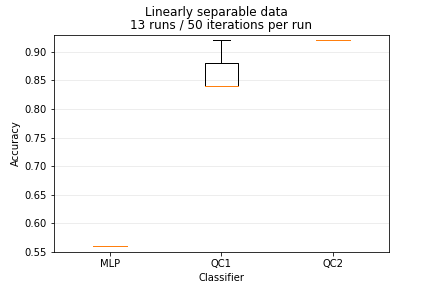
\includegraphics{Appendices/chapter_5/1qubit_Linearly_separable_data_13runs_50.png}
            }
        \end{subfigure}
        \begin{subfigure}{1.0\textwidth}
            \centering
            \scalebox{0.45}{
                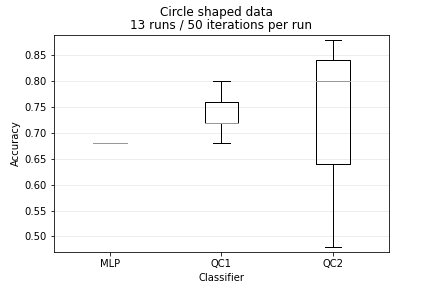
\includegraphics{Appendices/chapter_5/1qubit_Circle_shaped_data_13runs_50.png}
            }
        \end{subfigure}
        \begin{subfigure}{1.0\textwidth}
            \centering
            \scalebox{0.45}{
                 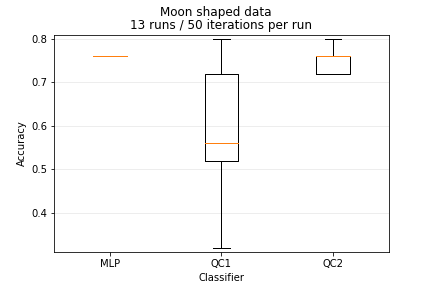
\includegraphics{Appendices/chapter_5/1qubit_Moon_shaped_data_13runs_50.png}
            }
        \end{subfigure}
        \caption{Accuracy box plots: \textbf{50 iterations} for all classifiers using \textbf{single qubit quantum circuits}.\\ \textbf{MLP}, \textbf{QC1} and \textbf{QC2} are referring to \textbf{Multi-layer Perceptron classifier}, \textbf{Quantum Circuit classifier 1} and \textbf{Quantum Circuit classifier 2} in figure \ref{fig:SingleQubitClassifiers_50Iterations} accordingly.}
        \label{fig:SingleQubitClassifiers_50Iterations_boxplot}
    \end{subfigure}
\end{figure}

\newpage
\begin{figure}[h!]
    \centering
    \caption{Decision boundary and accuracy comparison between Multi-layer Perceptron classifier, Quantum Circuit classifier 1 and Quantum Circuit classifier 2.\\\textit{Row 1}: Linearly separable data / \textit{Row 2}: Circle shaped data / \textit{Row 3}: Moon shaped data}
    \begin{subfigure}{1.0\textwidth}
        \centering
        \scalebox{0.27}{
            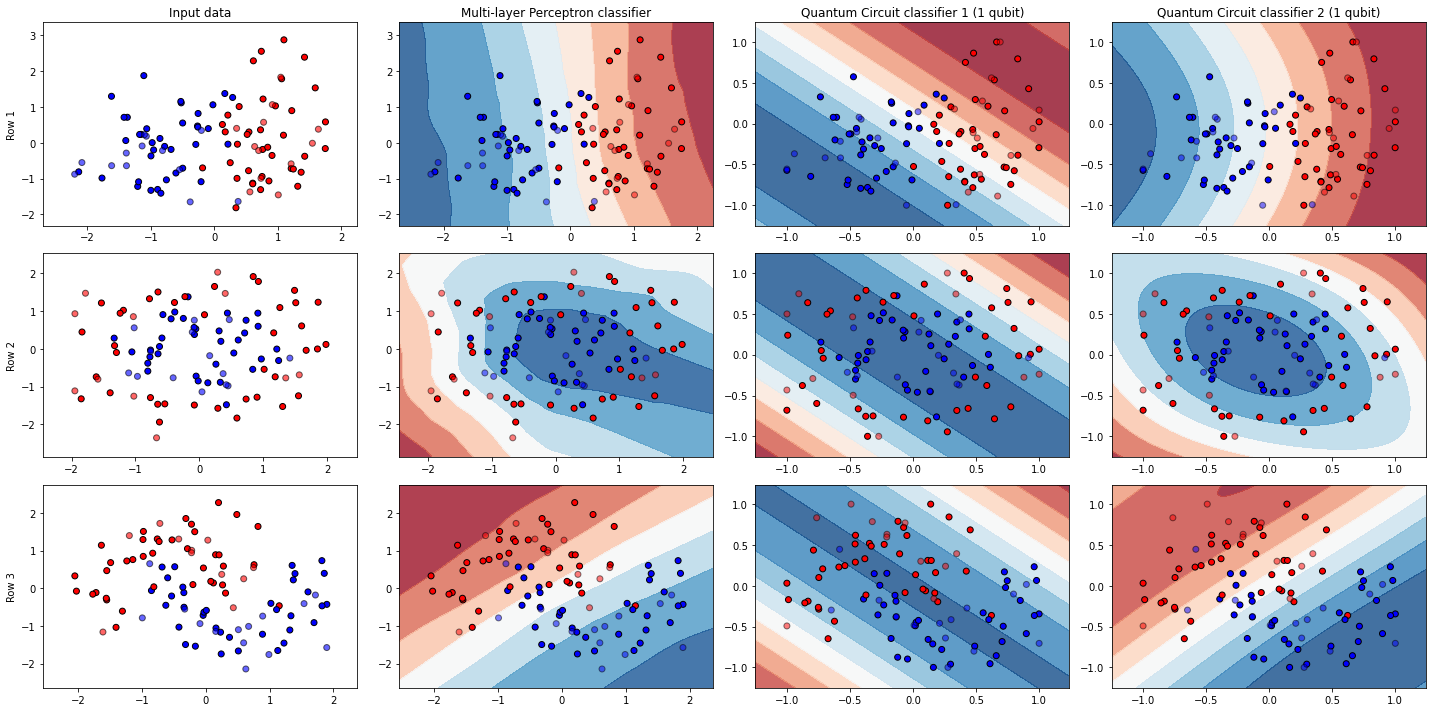
\includegraphics{Appendices/chapter_5/decision_boundary_1qubit_200-iter_01.png}
        }
        \caption{Decision boundary plot: \textbf{200 iterations} for all classifiers using \textbf{single qubit quantum circuits}.}
        \label{fig:SingleQubitClassifiers_200Iterations}
    \end{subfigure}
    \\[1ex]
    \begin{subfigure}{1.0\textwidth}
        \centering
        \begin{subfigure}{1.0\textwidth}
            \centering
            \scalebox{0.45}{
                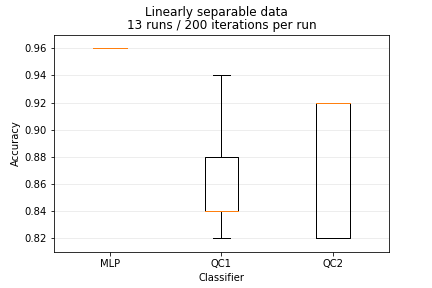
\includegraphics{Appendices/chapter_5/1qubit_Linearly_separable_data_13runs_200.png}
            }
        \end{subfigure}
        \begin{subfigure}{1.0\textwidth}
            \centering
            \scalebox{0.45}{
                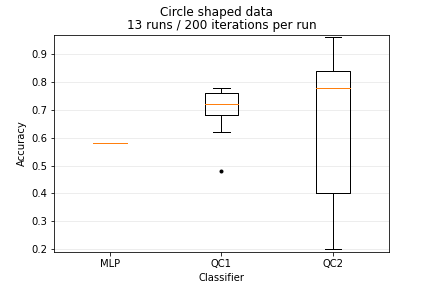
\includegraphics{Appendices/chapter_5/1qubit_Circle_shaped_data_13runs_200.png}
            }
        \end{subfigure}
        \begin{subfigure}{1.0\textwidth}
            \centering
            \scalebox{0.45}{
                 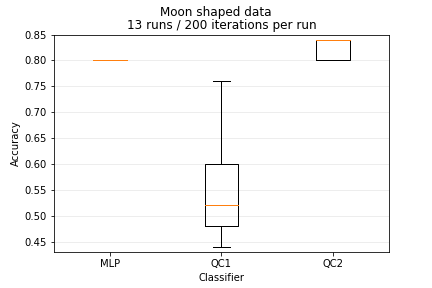
\includegraphics{Appendices/chapter_5/1qubit_Moon_shaped_data_13runs_200.png}
            }
        \end{subfigure}
        \caption{Accuracy box plots: \textbf{200 iterations} for all classifiers using \textbf{single qubit quantum circuits}.\\ \textbf{MLP}, \textbf{QC1} and \textbf{QC2} are referring to \textbf{Multi-layer Perceptron classifier}, \textbf{Quantum Circuit classifier 1} and \textbf{Quantum Circuit classifier 2} in figure \ref{fig:SingleQubitClassifiers_200Iterations} accordingly.}
        \label{fig:SingleQubitClassifiers_200Iterations_boxplot}
    \end{subfigure}
\end{figure}

\newpage
\begin{figure}[h!]
    \centering
    \caption{Decision boundary and accuracy comparison between Multi-layer Perceptron classifier, Quantum Circuit classifier 1 and Quantum Circuit classifier 2.\\\textit{Row 1}: Linearly separable data / \textit{Row 2}: Circle shaped data / \textit{Row 3}: Moon shaped data}
    \begin{subfigure}{1.0\textwidth}
        \centering
        \scalebox{0.27}{
            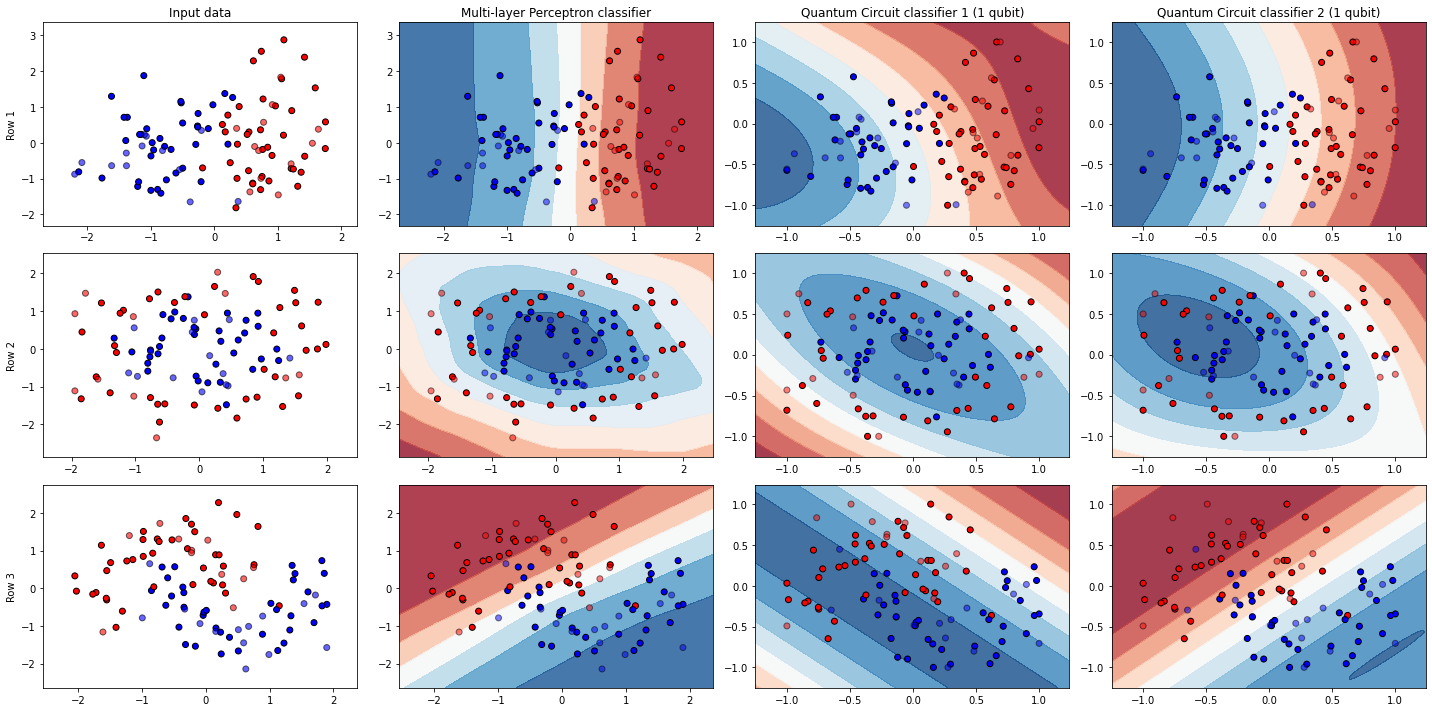
\includegraphics{Appendices/chapter_5/decision_boundary_1qubit_400-iter_01.png}
        }
        \caption{Decision boundary plot: \textbf{400 iterations} for all classifiers using \textbf{single qubit quantum circuits}.}
        \label{fig:SingleQubitClassifiers_400Iterations}
    \end{subfigure}
    \\[1ex]
    \begin{subfigure}{1.0\textwidth}
        \centering
        \begin{subfigure}{1.0\textwidth}
            \centering
            \scalebox{0.45}{
                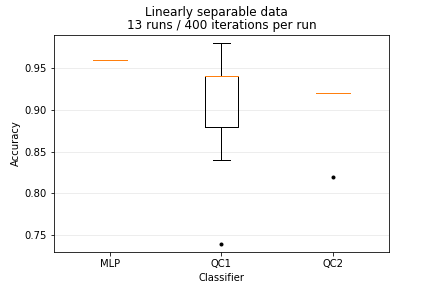
\includegraphics{Appendices/chapter_5/1qubit_Linearly_separable_data_13runs_400.png}
            }
        \end{subfigure}
        \begin{subfigure}{1.0\textwidth}
            \centering
            \scalebox{0.45}{
                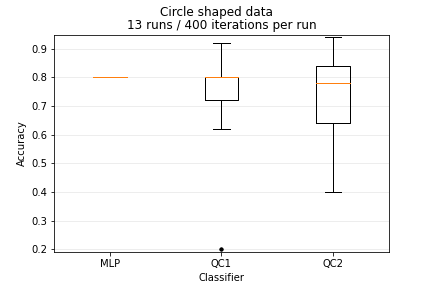
\includegraphics{Appendices/chapter_5/1qubit_Circle_shaped_data_13runs_400.png}
            }
        \end{subfigure}
        \begin{subfigure}{1.0\textwidth}
            \centering
            \scalebox{0.45}{
                 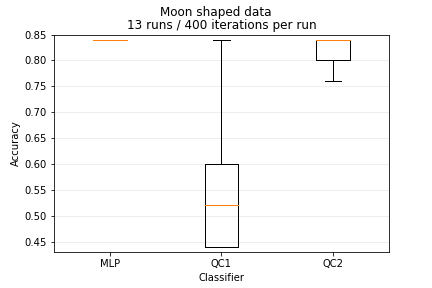
\includegraphics{Appendices/chapter_5/1qubit_Moon_shaped_data_13runs_400.png}
            }
        \end{subfigure}
        \caption{Accuracy box plots: \textbf{400 iterations} for all classifiers using \textbf{single qubit quantum circuits}.\\ \textbf{MLP}, \textbf{QC1} and \textbf{QC2} are referring to \textbf{Multi-layer Perceptron classifier}, \textbf{Quantum Circuit classifier 1} and \textbf{Quantum Circuit classifier 2} in figure \ref{fig:SingleQubitClassifiers_400Iterations} accordingly.}
        \label{fig:SingleQubitClassifiers_400Iterations_boxplot}
    \end{subfigure}
\end{figure}

\clearpage
\subsection{Two qubit circuits}
\label{subsection:two_qubit_circuits}
In this subsection, three two qubit quantum classifiers with angle embedding and a total count of six weights are trained. For comparison, there is also a Multi-layer Perceptron classifier (sklearn neural network \href{https://scikit-learn.org/stable/modules/generated/sklearn.neural_network.MLPClassifier.html}{MLPClassifier}) in the plots with the same iteration count as the quantum classifiers. Figure \ref{fig:2QubitClassifiers_50Iterations} has an iteration count of 50, figure \ref{fig:2QubitClassifiers_200Iterations} shows 200 iterations and the last figure \ref{fig:2QubitClassifiers_400Iterations} shows the classifiers after 400 iterations. The two qubit quantum classifier circuits can be seen in figures \ref{fig:two_qubit_circuit_1}, \ref{fig:two_qubit_circuit_2} and \ref{fig:two_qubit_circuit_3}.\\
\\

\begin{figure}[!h]
    \centering
    
    \begin{subfigure}{1.0\textwidth}
        \centering
        \scalebox{0.66}{
            \Qcircuit @C=1.0em @R=0.2em @!R { \\
            	 	\nghost{ {q}_{0} :  } & \lstick{ {q}_{0} :  } & \gate{\mathrm{H}} & \gate{\mathrm{R_Y}\,(\mathrm{\color{magenta}x_0})} & \ctrl{1} & \gate{\mathrm{R_Z}\,(\mathrm{\color{gray}w_0})} & \gate{\mathrm{R_Y}\,(\mathrm{\color{gray}w_1})} & \gate{\mathrm{R_Z}\,(\mathrm{\color{gray}w_2})} & \ctrl{1} & \qw & \qw\\ 
            	 	\nghost{ {q}_{1} :  } & \lstick{ {q}_{1} :  } & \gate{\mathrm{H}} & \gate{\mathrm{R_Y}\,(\mathrm{\color{magenta}x_1})} & \targ & \gate{\mathrm{R_Z}\,(\mathrm{\color{gray}w_3})} & \gate{\mathrm{R_Y}\,(\mathrm{\color{gray}w_4})} & \gate{\mathrm{R_Z}\,(\mathrm{\color{gray}w_5})} & \targ & \qw & \qw\\ 
            \\ }
        }
        \caption{\textbf{Quantum Circuit classifier 1} with starting Hadamard ($\mathrm{H}$) gates and angle embedding using a $\mathrm{RY}$ gates entangled with a $\mathrm{CX}$ gate followed by multiple $\mathrm{RY}$ and $\mathrm{RZ}$ rotation gates containing six weights in total, entangled with a final $\mathrm{CX}$ gate}
        \label{fig:two_qubit_circuit_1}
    \end{subfigure}
    \\[2ex]
    \begin{subfigure}{1.0\textwidth}
        \centering
        \scalebox{0.66}{
            \Qcircuit @C=1.0em @R=0.2em @!R { \\
            	 	\nghost{ {q}_{0} :  } & \lstick{ {q}_{0} :  } & \gate{\mathrm{H}} & \gate{\mathrm{R_Y}\,(\mathrm{\color{magenta}x_0})} & \gate{\mathrm{R_X}\,(\mathrm{\color{magenta}x_1})} & \ctrl{1} & \gate{\mathrm{R_Z}\,(\mathrm{\color{gray}w_0})} & \gate{\mathrm{R_Y}\,(\mathrm{\color{gray}w_1})} & \gate{\mathrm{R_Z}\,(\mathrm{\color{gray}w_2})} & \ctrl{1} & \qw & \qw\\ 
            	 	\nghost{ {q}_{1} :  } & \lstick{ {q}_{1} :  } & \gate{\mathrm{H}} & \qw & \qw & \targ & \gate{\mathrm{R_Z}\,(\mathrm{\color{gray}w_3})} & \gate{\mathrm{R_Y}\,(\mathrm{\color{gray}w_4})} & \gate{\mathrm{R_Z}\,(\mathrm{\color{gray}w_5})} & \targ & \qw & \qw\\ 
            \\ }
        }
        \caption{\textbf{Quantum Circuit classifier 2} differs from \textbf{Quantum Circuit classifier 1} \ref{fig:two_qubit_circuit_1} in terms of angle embedding using a $\mathrm{RY}$ and a $\mathrm{RX}$ gate to encode both features $x_0$, $x_1$ on the first qubit $q_0$ instead of using both qubits}
        \label{fig:two_qubit_circuit_2}
    \end{subfigure}
    \\[2ex]
    \begin{subfigure}{1.0\textwidth}
        \centering
        \scalebox{0.66}{
            \Qcircuit @C=1.0em @R=0.2em @!R { \\
        	 	\nghost{ {q}_{0} :  } & \lstick{ {q}_{0} :  } & \gate{\mathrm{H}} & \gate{\mathrm{R_Y}\,(\mathrm{\color{magenta}x_0})} & \ctrl{1} & \gate{\mathrm{R_Z}\,(\mathrm{\color{gray}w_0})} & \gate{\mathrm{R_Y}\,(\mathrm{\color{gray}w_1})} & \gate{\mathrm{R_Z}\,(\mathrm{\color{gray}w_2})} & \ctrl{1} & \qw & \qw\\ 
        	 	\nghost{ {q}_{1} :  } & \lstick{ {q}_{1} :  } & \gate{\mathrm{H}} & \gate{\mathrm{R_X}\,(\mathrm{\color{magenta}x_1})} & \targ & \gate{\mathrm{R_Z}\,(\mathrm{\color{gray}w_3})} & \gate{\mathrm{R_Y}\,(\mathrm{\color{gray}w_4})} & \gate{\mathrm{R_Z}\,(\mathrm{\color{gray}w_5})} & \targ & \qw & \qw\\ 
            \\ }
        }
        \caption{\textbf{Quantum Circuit classifier 3} with starting Hadamard ($\mathrm{H}$) gates and angle embedding using a $\mathrm{RY}$ and a $\mathrm{RX}$ gate}
        \label{fig:two_qubit_circuit_3}
    \end{subfigure}
    
    \caption{Two qubit quantum circuits referring to the \textbf{Quantum Circuit classifier 1}, \textbf{Quantum Circuit classifier 2} and \textbf{Quantum Circuit classifier 3} in figures \ref{fig:2QubitClassifiers_50Iterations}, \ref{fig:2QubitClassifiers_200Iterations} and \ref{fig:2QubitClassifiers_400Iterations}.}
    \label{fig:two_qubit_circuits}
\end{figure}

% Contour and box plots
\begin{figure}[!h]
    \centering
    \caption{Decision boundary and accuracy comparison between Multi-layer Perceptron classifier, Quantum Circuit classifier 1, Quantum Circuit classifier 2 and Quantum Circuit classifier 3.\\\textit{Row 1}: Linearly separable data / \textit{Row 2}: Circle shaped data / \textit{Row 3}: Moon shaped data}
    \begin{subfigure}{1.0\textwidth}
        \centering
        \scalebox{0.27}{
            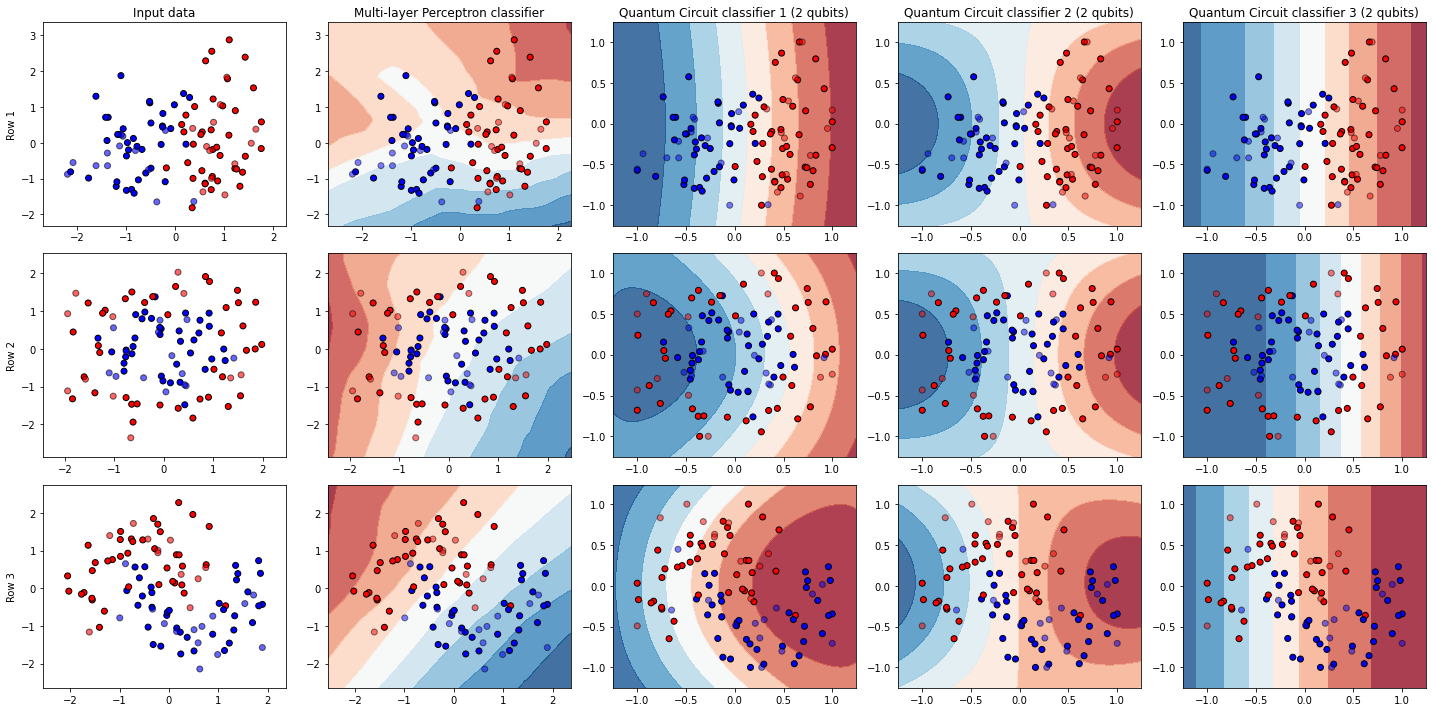
\includegraphics{Appendices/chapter_5/decision_boundary_2qubits_50-iter_01.png}
        }
        \caption{\textbf{50 iterations} for all classifiers using \textbf{two qubit quantum circuits}.}
        \label{fig:2QubitClassifiers_50Iterations}
    \end{subfigure}
    \\[1ex]
    \begin{subfigure}{1.0\textwidth}
        \centering
        \begin{subfigure}{1.0\textwidth}
            \centering
            \scalebox{0.45}{
                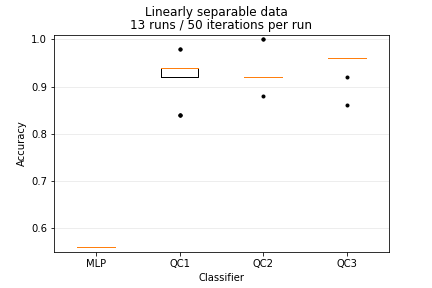
\includegraphics{Appendices/chapter_5/2qubits_Linearly_separable_data_13runs_50.png}
            }
        \end{subfigure}
        \begin{subfigure}{1.0\textwidth}
            \centering
            \scalebox{0.45}{
                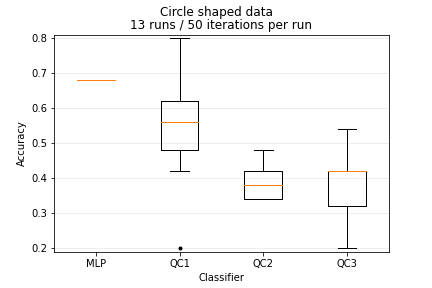
\includegraphics{Appendices/chapter_5/2qubits_Circle_shaped_data_13runs_50.png}
            }
        \end{subfigure}
        \begin{subfigure}{1.0\textwidth}
            \centering
            \scalebox{0.45}{
                 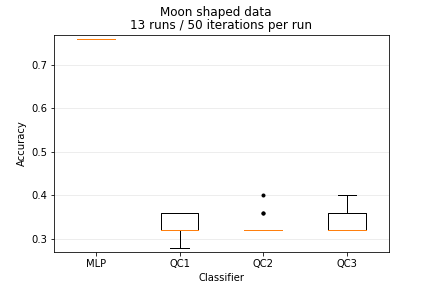
\includegraphics{Appendices/chapter_5/2qubits_Moon_shaped_data_13runs_50.png}
            }
        \end{subfigure}
        \caption{Accuracy box plots: \textbf{50 iterations} for all classifiers using \textbf{two qubit quantum circuits}.\\ \textbf{MLP}, \textbf{QC1}, \textbf{QC2} and \textbf{QC3} are referring to \textbf{Multi-layer Perceptron classifier}, \textbf{Quantum Circuit classifier 1}, \textbf{Quantum Circuit classifier 2} and \textbf{Quantum Circuit classifier 3} in figure \ref{fig:2QubitClassifiers_50Iterations} accordingly.}
        \label{fig:2QubitClassifiers_50Iterations_boxplot}
    \end{subfigure}
\end{figure}

\newpage
\begin{figure}[!h]
    \centering
    \caption{Decision boundary and accuracy comparison between Multi-layer Perceptron classifier, Quantum Circuit classifier 1, Quantum Circuit classifier 2 and Quantum Circuit classifier 3.\\\textit{Row 1}: Linearly separable data / \textit{Row 2}: Circle shaped data / \textit{Row 3}: Moon shaped data}
    \begin{subfigure}{1.0\textwidth}
        \centering
        \scalebox{0.27}{
            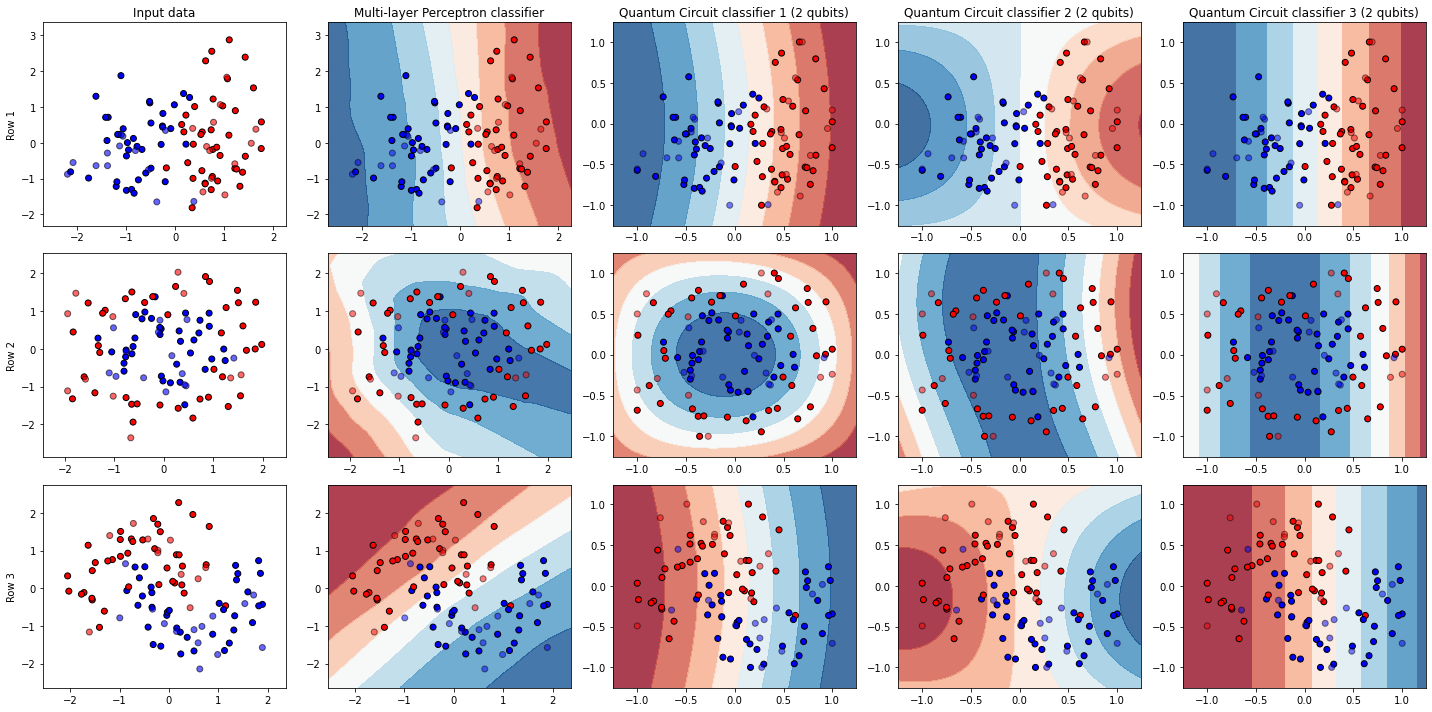
\includegraphics{Appendices/chapter_5/decision_boundary_2qubits_200-iter_01.png}
        }
        \caption{\textbf{200 iterations} for all classifiers using \textbf{two qubit quantum circuits}.}
        \label{fig:2QubitClassifiers_200Iterations}
    \end{subfigure}
    \\[1ex]
    \begin{subfigure}{1.0\textwidth}
        \centering
        \begin{subfigure}{1.0\textwidth}
            \centering
            \scalebox{0.45}{
                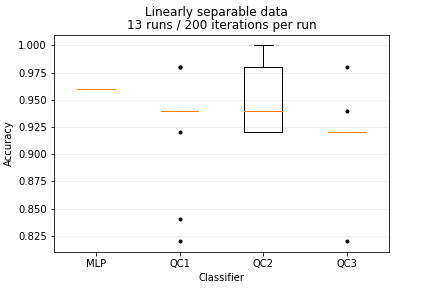
\includegraphics{Appendices/chapter_5/2qubits_Linearly_separable_data_13runs_200.png}
            }
        \end{subfigure}
        \begin{subfigure}{1.0\textwidth}
            \centering
            \scalebox{0.45}{
                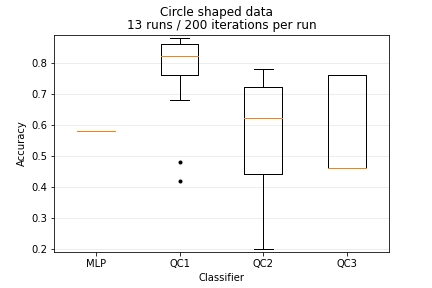
\includegraphics{Appendices/chapter_5/2qubits_Circle_shaped_data_13runs_200.png}
            }
        \end{subfigure}
        \begin{subfigure}{1.0\textwidth}
            \centering
            \scalebox{0.45}{
                 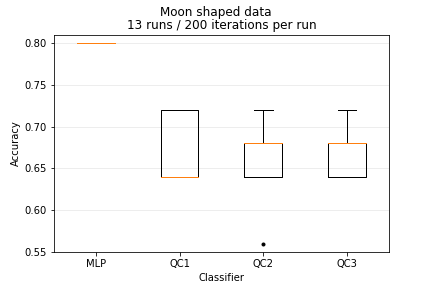
\includegraphics{Appendices/chapter_5/2qubits_Moon_shaped_data_13runs_200.png}
            }
        \end{subfigure}
        \caption{Accuracy box plots: \textbf{200 iterations} for all classifiers using \textbf{two qubit quantum circuits}.\\ \textbf{MLP}, \textbf{QC1}, \textbf{QC2} and \textbf{QC3} are referring to \textbf{Multi-layer Perceptron classifier}, \textbf{Quantum Circuit classifier 1}, \textbf{Quantum Circuit classifier 2} and \textbf{Quantum Circuit classifier 3} in figure \ref{fig:2QubitClassifiers_200Iterations} accordingly.}
        \label{fig:2QubitClassifiers_200Iterations_boxplot}
    \end{subfigure}
\end{figure}

\newpage
\begin{figure}[!h]
    \centering
    \caption{Decision boundary and accuracy comparison between Multi-layer Perceptron classifier, Quantum Circuit classifier 1, Quantum Circuit classifier 2 and Quantum Circuit classifier 3.\\\textit{Row 1}: Linearly separable data / \textit{Row 2}: Circle shaped data / \textit{Row 3}: Moon shaped data}
    \begin{subfigure}{1.0\textwidth}
        \centering
        \scalebox{0.27}{
            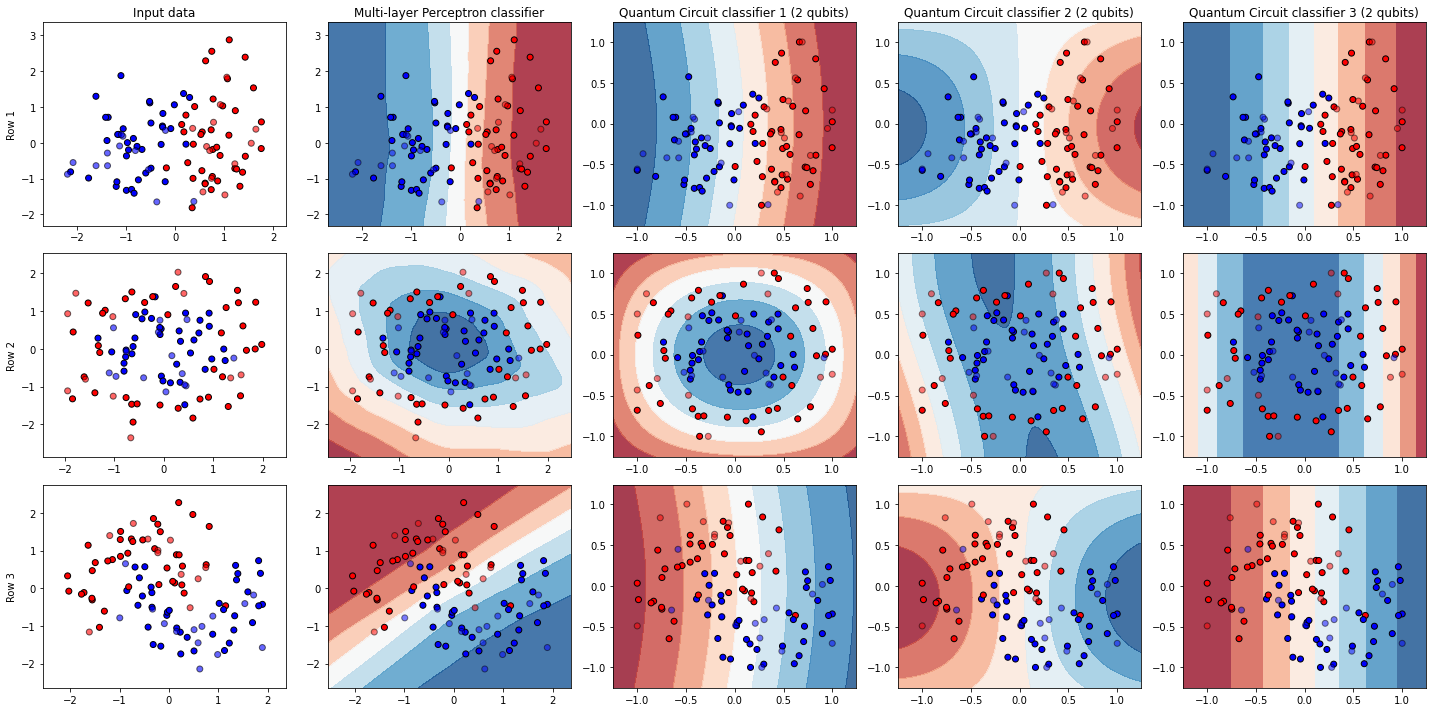
\includegraphics{Appendices/chapter_5/decision_boundary_2qubits_400-iter_01.png}
        }
        \caption{\textbf{400 iterations} for all classifiers using \textbf{two qubit quantum circuits}.}
        \label{fig:2QubitClassifiers_400Iterations}
    \end{subfigure}
    \\[1ex]
    \begin{subfigure}{1.0\textwidth}
        \centering
        \begin{subfigure}{1.0\textwidth}
            \centering
            \scalebox{0.45}{
                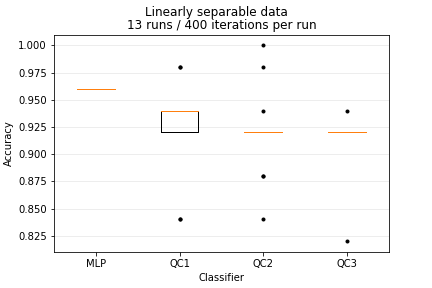
\includegraphics{Appendices/chapter_5/2qubits_Linearly_separable_data_13runs_400.png}
            }
        \end{subfigure}
        \begin{subfigure}{1.0\textwidth}
            \centering
            \scalebox{0.45}{
                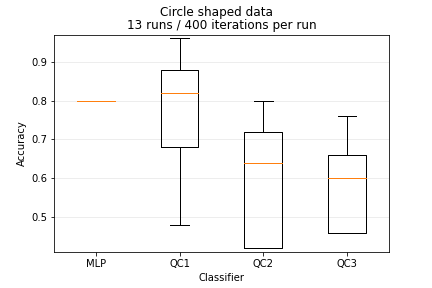
\includegraphics{Appendices/chapter_5/2qubits_Circle_shaped_data_13runs_400.png}
            }
        \end{subfigure}
        \begin{subfigure}{1.0\textwidth}
            \centering
            \scalebox{0.45}{
                 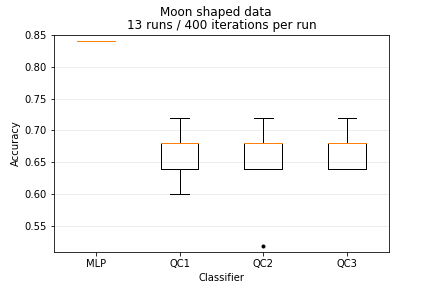
\includegraphics{Appendices/chapter_5/2qubits_Moon_shaped_data_13runs_400.png}
            }
        \end{subfigure}
        \caption{Accuracy box plots: \textbf{400 iterations} for all classifiers using \textbf{two qubit quantum circuits}.\\ \textbf{MLP}, \textbf{QC1}, \textbf{QC2} and \textbf{QC3} are referring to \textbf{Multi-layer Perceptron classifier}, \textbf{Quantum Circuit classifier 1}, \textbf{Quantum Circuit classifier 2} and \textbf{Quantum Circuit classifier 3} in figure \ref{fig:2QubitClassifiers_400Iterations} accordingly.}
        \label{fig:2QubitClassifiers_400Iterations_boxplot}
    \end{subfigure}
\end{figure}

\clearpage
\subsection{Two qubit circuits with 3 layers}
\label{subsection:two_qubit_circuits_3layers}

In this subsection, three two qubit quantum classifiers with three layers (the same quantum circuits as in subsection \ref{subsection:two_qubit_circuits} repeated three times, excluding the Hadamard ($\mathrm{H}$) gates) using angle embedding and a total count of $3\times6 = 18$ weights have been trained. Again for comparison, there is also a Multi-layer Perceptron classifier (sklearn neural network \href{https://scikit-learn.org/stable/modules/generated/sklearn.neural_network.MLPClassifier.html}{MLPClassifier}) in the plots with the same iteration count as the quantum classifiers, but this time with 3 hidden layers as seen in figure \ref{fig:code_MLPClassifier_configuration_3hiddenlayers}. Figure \ref{fig:2Qubit3LayersClassifiers_50Iterations} has an iteration count of 50, figure \ref{fig:2Qubit3LayersClassifiers_200Iterations} shows 200 iterations and the last figure \ref{fig:2Qubit3LayersClassifiers_400Iterations} shows the classifiers after 400 iterations. The two qubit quantum classifiers with three layer circuits can be seen in figures \ref{fig:two_qubit_3layers_circuit_1}, \ref{fig:two_qubit_3layers_circuit_2} and \ref{fig:two_qubit_3layers_circuit_3}.\\

\hfill \break

\begin{figure}[!h]
    \centering
    
    \begin{subfigure}{1.0\textwidth}
        \centering
        \scalebox{0.43}{
            \Qcircuit @C=1.0em @R=0.2em @!R { \\
            	 	\nghost{ {q}_{0} :  } & \lstick{ {q}_{0} :  } & \gate{\mathrm{H}} \barrier[0em]{1} & \qw & \gate{\mathrm{R_Y}\,(\mathrm{\color{magenta}x_0})} & \ctrl{1} & \gate{\mathrm{R_Z}\,(\mathrm{\color{gray}w_0})} & \gate{\mathrm{R_Y}\,(\mathrm{\color{gray}w_1})} & \gate{\mathrm{R_Z}\,(\mathrm{\color{gray}w_2})} & \ctrl{1} \barrier[0em]{1} & \qw & \gate{\mathrm{R_Y}\,(\mathrm{\color{magenta}x_0})} & \ctrl{1} & \gate{\mathrm{R_Z}\,(\mathrm{\color{gray}w_6})} & \gate{\mathrm{R_Y}\,(\mathrm{\color{gray}w_7})} & \gate{\mathrm{R_Z}\,(\mathrm{\color{gray}w_8})} & \ctrl{1} \barrier[0em]{1} & \qw & \gate{\mathrm{R_Y}\,(\mathrm{\color{magenta}x_0})} & \ctrl{1} & \gate{\mathrm{R_Z}\,(\mathrm{\color{gray}w_{12}})} & \gate{\mathrm{R_Y}\,(\mathrm{\color{gray}w_{13}})} & \gate{\mathrm{R_Z}\,(\mathrm{\color{gray}w_{14}})} & \ctrl{1} & \qw & \qw\\ 
            	 	\nghost{ {q}_{1} :  } & \lstick{ {q}_{1} :  } & \gate{\mathrm{H}} & \qw & \gate{\mathrm{R_Y}\,(\mathrm{\color{magenta}x_1})} & \targ & \gate{\mathrm{R_Z}\,(\mathrm{\color{gray}w_3})} & \gate{\mathrm{R_Y}\,(\mathrm{\color{gray}w_4})} & \gate{\mathrm{R_Z}\,(\mathrm{\color{gray}w_5})} & \targ & \qw & \gate{\mathrm{R_Y}\,(\mathrm{\color{magenta}x_1})} & \targ & \gate{\mathrm{R_Z}\,(\mathrm{\color{gray}w_9})} & \gate{\mathrm{R_Y}\,(\mathrm{\color{gray}w_{10}})} & \gate{\mathrm{R_Z}\,(\mathrm{\color{gray}w_{11}})} & \targ & \qw & \gate{\mathrm{R_Y}\,(\mathrm{\color{magenta}x_1})} & \targ & \gate{\mathrm{R_Z}\,(\mathrm{\color{gray}w_{15}})} & \gate{\mathrm{R_Y}\,(\mathrm{\color{gray}w_{16}})} & \gate{\mathrm{R_Z}\,(\mathrm{\color{gray}w_{17}})} & \targ & \qw & \qw\\ 
            \\ }
        }
        \caption{\textbf{Quantum Circuit classifier 1} same as the two qubit classifier in figure \ref{fig:two_qubit_circuit_1} with 2 additional "layers"}
        \label{fig:two_qubit_3layers_circuit_1}
    \end{subfigure}
    \\[2ex]
    \begin{subfigure}{1.0\textwidth}
        \centering
        \scalebox{0.37}{
            \Qcircuit @C=1.0em @R=0.2em @!R { \\
            	 	\nghost{ {q}_{0} :  } & \lstick{ {q}_{0} :  } & \gate{\mathrm{H}} \barrier[0em]{1} & \qw & \gate{\mathrm{R_Y}\,(\mathrm{\color{magenta}x_0})} & \gate{\mathrm{R_X}\,(\mathrm{\color{magenta}x_1})} & \ctrl{1} & \gate{\mathrm{R_Z}\,(\mathrm{\color{gray}w_0})} & \gate{\mathrm{R_Y}\,(\mathrm{\color{gray}w_1})} & \gate{\mathrm{R_Z}\,(\mathrm{\color{gray}w_2})} & \ctrl{1} \barrier[0em]{1} & \qw & \gate{\mathrm{R_Y}\,(\mathrm{\color{magenta}x_0})} & \gate{\mathrm{R_X}\,(\mathrm{\color{magenta}x_1})} & \ctrl{1} & \gate{\mathrm{R_Z}\,(\mathrm{\color{gray}w_6})} & \gate{\mathrm{R_Y}\,(\mathrm{\color{gray}w_7})} & \gate{\mathrm{R_Z}\,(\mathrm{\color{gray}w_8})} & \ctrl{1} \barrier[0em]{1} & \qw & \gate{\mathrm{R_Y}\,(\mathrm{\color{magenta}x_0})} & \gate{\mathrm{R_X}\,(\mathrm{\color{magenta}x_1})} & \ctrl{1} & \gate{\mathrm{R_Z}\,(\mathrm{\color{gray}w_{12}})} & \gate{\mathrm{R_Y}\,(\mathrm{\color{gray}w_{13}})} & \gate{\mathrm{R_Z}\,(\mathrm{\color{gray}w_{14}})} & \ctrl{1} & \qw & \qw\\ 
            	 	\nghost{ {q}_{1} :  } & \lstick{ {q}_{1} :  } & \gate{\mathrm{H}} & \qw & \qw & \qw & \targ & \gate{\mathrm{R_Z}\,(\mathrm{\color{gray}w_3})} & \gate{\mathrm{R_Y}\,(\mathrm{\color{gray}w_4})} & \gate{\mathrm{R_Z}\,(\mathrm{\color{gray}w_5})} & \targ & \qw & \qw & \qw & \targ & \gate{\mathrm{R_Z}\,(\mathrm{\color{gray}w_9})} & \gate{\mathrm{R_Y}\,(\mathrm{\color{gray}w_{10}})} & \gate{\mathrm{R_Z}\,(\mathrm{\color{gray}w_{11}})} & \targ & \qw & \qw & \qw & \targ & \gate{\mathrm{R_Z}\,(\mathrm{\color{gray}w_{15}})} & \gate{\mathrm{R_Y}\,(\mathrm{\color{gray}w_{16}})} & \gate{\mathrm{R_Z}\,(\mathrm{\color{gray}w_{17}})} & \targ & \qw & \qw\\ 
            \\ }
        }
        \caption{\textbf{Quantum Circuit classifier 2} same as the two qubit classifier in figure \ref{fig:two_qubit_circuit_2} with 2 additional "layers"}
        \label{fig:two_qubit_3layers_circuit_2}
    \end{subfigure}
    \\[2ex]
    \begin{subfigure}{1.0\textwidth}
        \centering
        \scalebox{0.43}{
            \Qcircuit @C=1.0em @R=0.2em @!R { \\
            	 	\nghost{ {q}_{0} :  } & \lstick{ {q}_{0} :  } & \gate{\mathrm{H}} \barrier[0em]{1} & \qw & \gate{\mathrm{R_Y}\,(\mathrm{\color{magenta}x_0})} & \ctrl{1} & \gate{\mathrm{R_Z}\,(\mathrm{\color{gray}w_0})} & \gate{\mathrm{R_Y}\,(\mathrm{\color{gray}w_1})} & \gate{\mathrm{R_Z}\,(\mathrm{\color{gray}w_2})} & \ctrl{1} \barrier[0em]{1} & \qw & \gate{\mathrm{R_Y}\,(\mathrm{\color{magenta}x_0})} & \ctrl{1} & \gate{\mathrm{R_Z}\,(\mathrm{\color{gray}w_6})} & \gate{\mathrm{R_Y}\,(\mathrm{\color{gray}w_7})} & \gate{\mathrm{R_Z}\,(\mathrm{\color{gray}w_8})} & \ctrl{1} \barrier[0em]{1} & \qw & \gate{\mathrm{R_Y}\,(\mathrm{\color{magenta}x_0})} & \ctrl{1} & \gate{\mathrm{R_Z}\,(\mathrm{\color{gray}w_{12}})} & \gate{\mathrm{R_Y}\,(\mathrm{\color{gray}w_{13}})} & \gate{\mathrm{R_Z}\,(\mathrm{\color{gray}w_{14}})} & \ctrl{1} & \qw & \qw\\ 
            	 	\nghost{ {q}_{1} :  } & \lstick{ {q}_{1} :  } & \gate{\mathrm{H}} & \qw & \gate{\mathrm{R_X}\,(\mathrm{\color{magenta}x_1})} & \targ & \gate{\mathrm{R_Z}\,(\mathrm{\color{gray}w_3})} & \gate{\mathrm{R_Y}\,(\mathrm{\color{gray}w_4})} & \gate{\mathrm{R_Z}\,(\mathrm{\color{gray}w_5})} & \targ & \qw & \gate{\mathrm{R_X}\,(\mathrm{\color{magenta}x_1})} & \targ & \gate{\mathrm{R_Z}\,(\mathrm{\color{gray}w_9})} & \gate{\mathrm{R_Y}\,(\mathrm{\color{gray}w_{10}})} & \gate{\mathrm{R_Z}\,(\mathrm{\color{gray}w_{11}})} & \targ & \qw & \gate{\mathrm{R_X}\,(\mathrm{\color{magenta}x_1})} & \targ & \gate{\mathrm{R_Z}\,(\mathrm{\color{gray}w_{15}})} & \gate{\mathrm{R_Y}\,(\mathrm{\color{gray}w_{16}})} & \gate{\mathrm{R_Z}\,(\mathrm{\color{gray}w_{17}})} & \targ & \qw & \qw\\ 
            \\ }
        }
        \caption{\textbf{Quantum Circuit classifier 3} same as the two qubit classifier in figure \ref{fig:two_qubit_circuit_3} with 2 additional "layers"}
        \label{fig:two_qubit_3layers_circuit_3}
    \end{subfigure}
    
    \caption{Two qubit quantum circuits with 3 layers referring to the \textbf{Quantum Circuit classifier 1}, \textbf{Quantum Circuit classifier 2} and \textbf{Quantum Circuit classifier 3} in figures \ref{fig:2Qubit3LayersClassifiers_50Iterations}, \ref{fig:2Qubit3LayersClassifiers_200Iterations} and \ref{fig:2Qubit3LayersClassifiers_400Iterations}. For better visual understanding three barriers have been added, marking the beginning of each layer. The barriers have no impact on the circuits themselves and are only used for visualization purposes.}
    \label{fig:two_qubit_3layers_circuits}
\end{figure}

% Contour and box plots
\begin{figure}[!h]
    \centering
    \caption{Decision boundary and accuracy comparison between Multi-layer Perceptron classifier, Quantum Circuit classifier 1, Quantum Circuit classifier 2 and Quantum Circuit classifier 3.\\\textit{Row 1}: Linearly separable data / \textit{Row 2}: Circle shaped data / \textit{Row 3}: Moon shaped data}
    \begin{subfigure}{1.0\textwidth}
        \centering
        \scalebox{0.27}{
            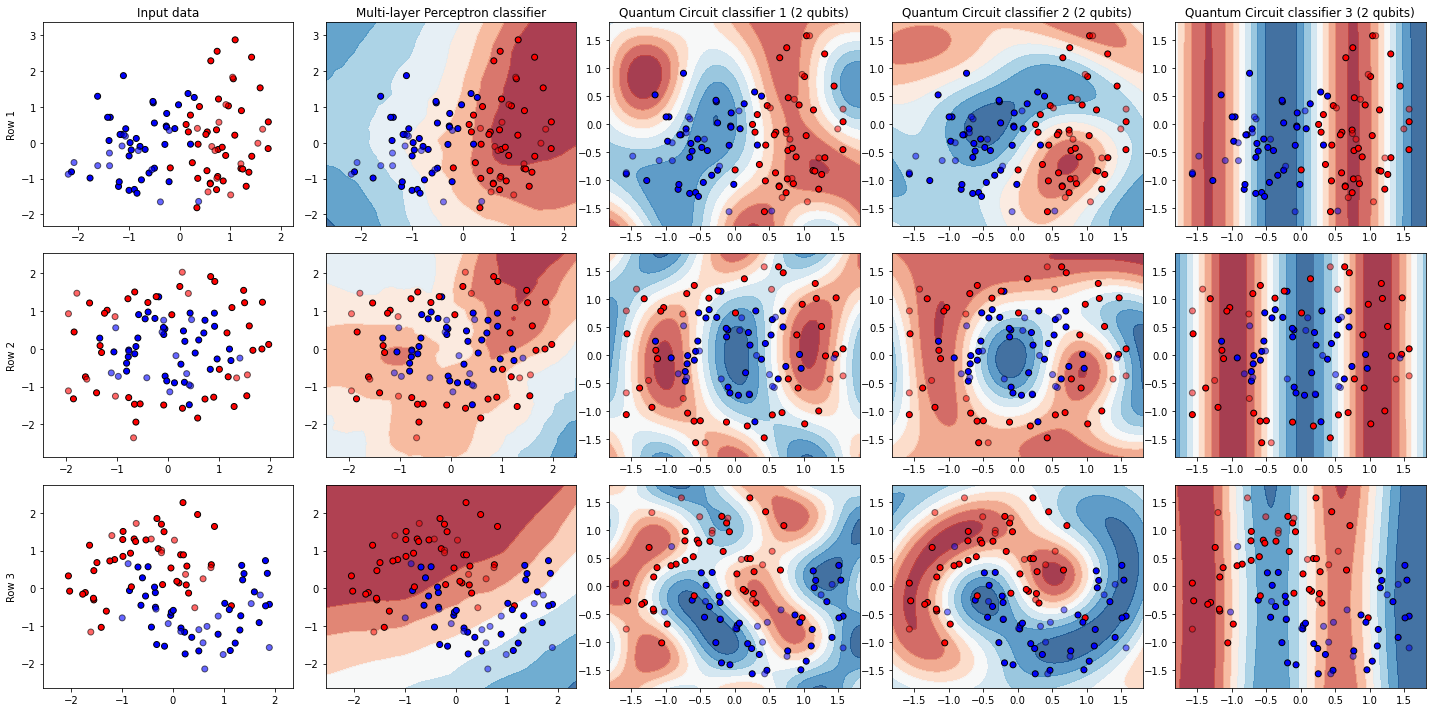
\includegraphics{Appendices/chapter_5/decision_boundary_2qubits_3layers_50-iter_01.png}
        }
        \caption{\textbf{50 iterations} for all classifiers using \textbf{two qubit quantum circuits with 3 layers}.}
        \label{fig:2Qubit3LayersClassifiers_50Iterations}
    \end{subfigure}
    \\[1ex]
    \begin{subfigure}{1.0\textwidth}
        \centering
        \begin{subfigure}{1.0\textwidth}
            \centering
            \scalebox{0.45}{
                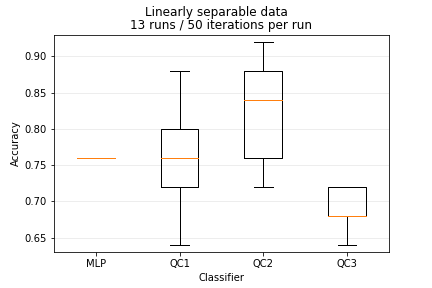
\includegraphics{Appendices/chapter_5/2qubits_3layers_Linearly_separable_data_13runs_50.png}
            }
        \end{subfigure}
        \begin{subfigure}{1.0\textwidth}
            \centering
            \scalebox{0.45}{
                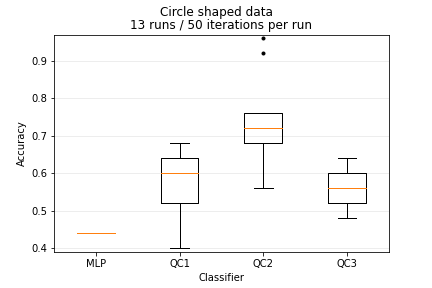
\includegraphics{Appendices/chapter_5/2qubits_3layers_Circle_shaped_data_13runs_50.png}
            }
        \end{subfigure}
        \begin{subfigure}{1.0\textwidth}
            \centering
            \scalebox{0.45}{
                 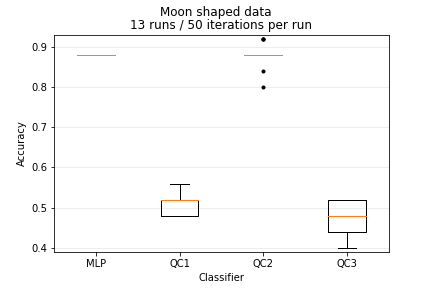
\includegraphics{Appendices/chapter_5/2qubits_3layers_Moon_shaped_data_13runs_50.png}
            }
        \end{subfigure}
        \caption{Accuracy box plots: \textbf{50 iterations} for all classifiers using \textbf{two qubit quantum circuits with 3 layers}.\\ \textbf{MLP}, \textbf{QC1}, \textbf{QC2} and \textbf{QC3} are referring to \textbf{Multi-layer Perceptron classifier}, \textbf{Quantum Circuit classifier 1}, \textbf{Quantum Circuit classifier 2} and \textbf{Quantum Circuit classifier 3} in figure \ref{fig:2Qubit3LayersClassifiers_50Iterations} accordingly.}
        \label{fig:2Qubit3LayersClassifiers_50Iterations_boxplot}
    \end{subfigure}
\end{figure}

\newpage
\begin{figure}[!h]
    \centering
    \caption{Decision boundary and accuracy comparison between Multi-layer Perceptron classifier, Quantum Circuit classifier 1, Quantum Circuit classifier 2 and Quantum Circuit classifier 3.\\\textit{Row 1}: Linearly separable data / \textit{Row 2}: Circle shaped data / \textit{Row 3}: Moon shaped data}
    \begin{subfigure}{1.0\textwidth}
        \centering
        \scalebox{0.27}{
            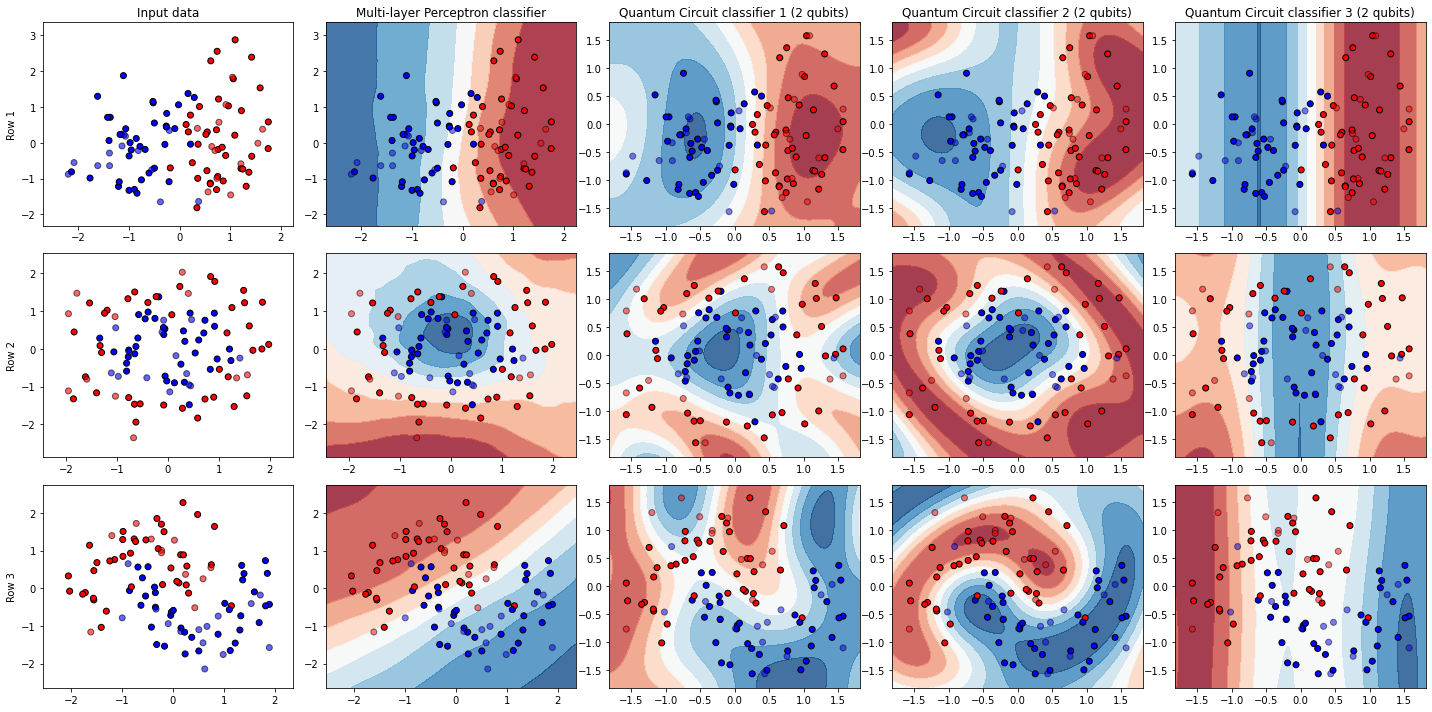
\includegraphics{Appendices/chapter_5/decision_boundary_2qubits_3layers_200-iter_01.png}
        }
        \caption{\textbf{200 iterations} for all classifiers using \textbf{two qubit quantum circuits with 3 layers}.}
        \label{fig:2Qubit3LayersClassifiers_200Iterations}
    \end{subfigure}
    \\[1ex]
    \begin{subfigure}{1.0\textwidth}
        \centering
        \begin{subfigure}{1.0\textwidth}
            \centering
            \scalebox{0.45}{
                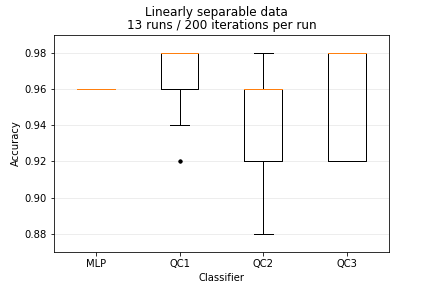
\includegraphics{Appendices/chapter_5/2qubits_3layers_Linearly_separable_data_13runs_200.png}
            }
        \end{subfigure}
        \begin{subfigure}{1.0\textwidth}
            \centering
            \scalebox{0.45}{
                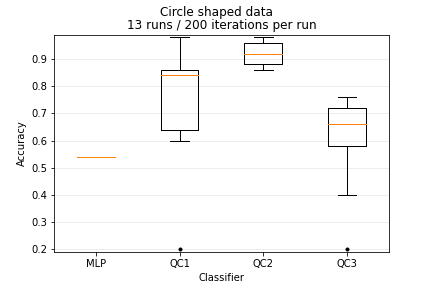
\includegraphics{Appendices/chapter_5/2qubits_3layers_Circle_shaped_data_13runs_200.png}
            }
        \end{subfigure}
        \begin{subfigure}{1.0\textwidth}
            \centering
            \scalebox{0.45}{
                 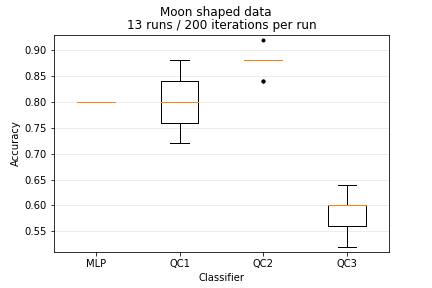
\includegraphics{Appendices/chapter_5/2qubits_3layers_Moon_shaped_data_13runs_200.png}
            }
        \end{subfigure}
        \caption{Accuracy box plots: \textbf{200 iterations} for all classifiers using \textbf{two qubit quantum circuits with 3 layers}.\\ \textbf{MLP}, \textbf{QC1}, \textbf{QC2} and \textbf{QC3} are referring to \textbf{Multi-layer Perceptron classifier}, \textbf{Quantum Circuit classifier 1}, \textbf{Quantum Circuit classifier 2} and \textbf{Quantum Circuit classifier 3} in figure \ref{fig:2Qubit3LayersClassifiers_200Iterations} accordingly.}
        \label{fig:2Qubit3LayersClassifiers_200Iterations_boxplot}
    \end{subfigure}
\end{figure}

\newpage
\begin{figure}[!h]
    \centering
    \caption{Decision boundary and accuracy comparison between Multi-layer Perceptron classifier, Quantum Circuit classifier 1, Quantum Circuit classifier 2 and Quantum Circuit classifier 3.\\\textit{Row 1}: Linearly separable data / \textit{Row 2}: Circle shaped data / \textit{Row 3}: Moon shaped data}
    \begin{subfigure}{1.0\textwidth}
        \centering
        \scalebox{0.27}{
            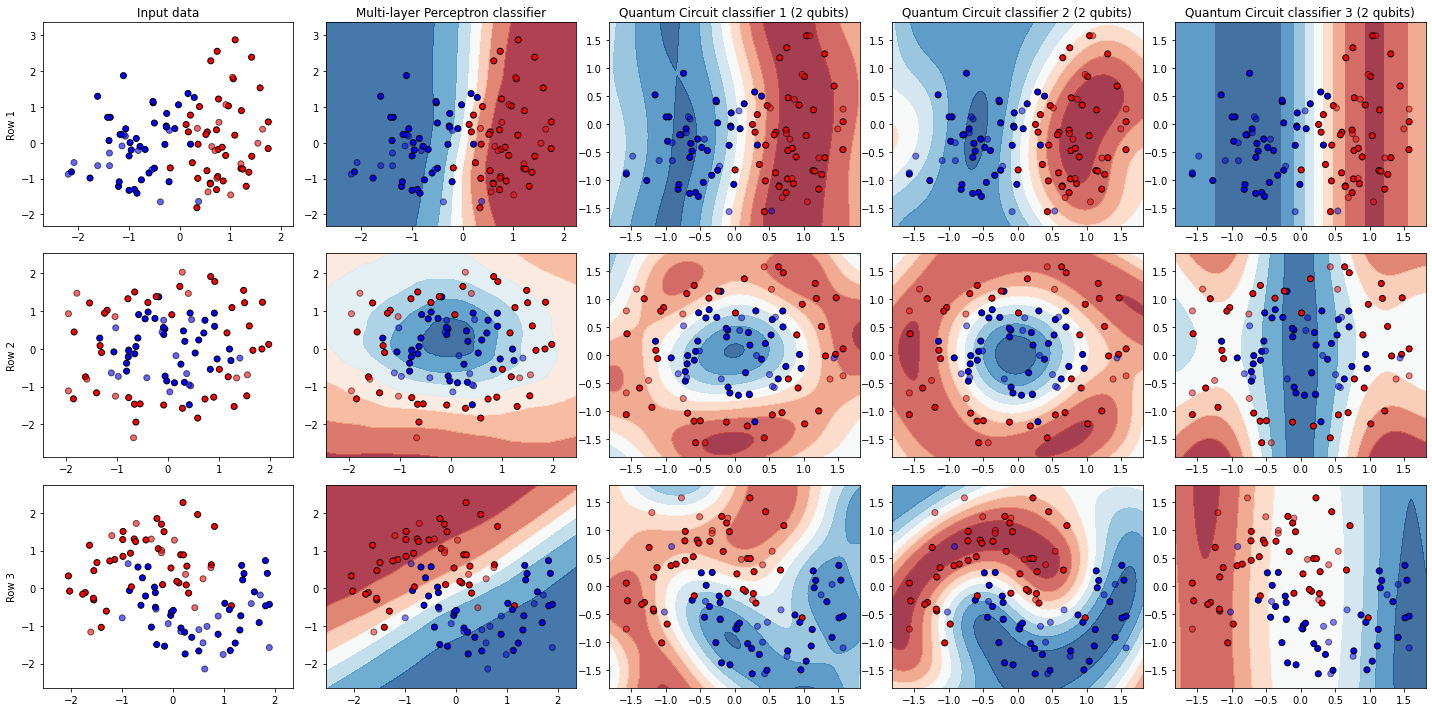
\includegraphics{Appendices/chapter_5/decision_boundary_2qubits_3layers_400-iter_01.png}
        }
        \caption{\textbf{400 iterations} for all classifiers using \textbf{two qubit quantum circuits with 3 layers}.}
        \label{fig:2Qubit3LayersClassifiers_400Iterations}
    \end{subfigure}
    \\[1ex]
    \begin{subfigure}{1.0\textwidth}
        \centering
        \begin{subfigure}{1.0\textwidth}
            \centering
            \scalebox{0.45}{
                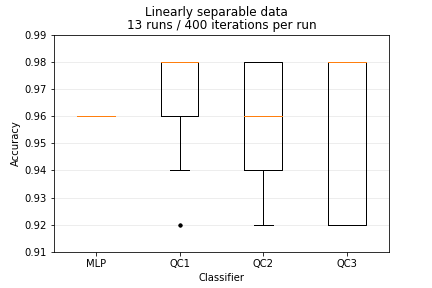
\includegraphics{Appendices/chapter_5/2qubits_3layers_Linearly_separable_data_13runs_400.png}
            }
        \end{subfigure}
        \begin{subfigure}{1.0\textwidth}
            \centering
            \scalebox{0.45}{
                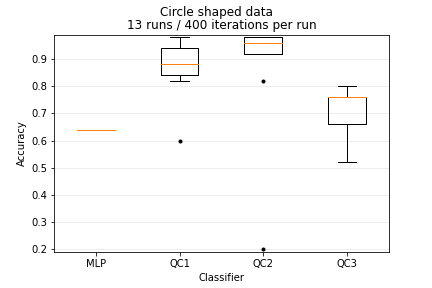
\includegraphics{Appendices/chapter_5/2qubits_3layers_Circle_shaped_data_13runs_400.png}
            }
        \end{subfigure}
        \begin{subfigure}{1.0\textwidth}
            \centering
            \scalebox{0.45}{
                 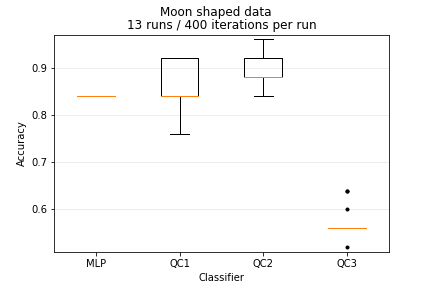
\includegraphics{Appendices/chapter_5/2qubits_3layers_Moon_shaped_data_13runs_400.png}
            }
        \end{subfigure}
        \caption{Accuracy box plots: \textbf{400 iterations} for all classifiers using \textbf{two qubit quantum circuits with 3 layers}.\\ \textbf{MLP}, \textbf{QC1}, \textbf{QC2} and \textbf{QC3} are referring to \textbf{Multi-layer Perceptron classifier}, \textbf{Quantum Circuit classifier 1}, \textbf{Quantum Circuit classifier 2} and \textbf{Quantum Circuit classifier 3} in figure \ref{fig:2Qubit3LayersClassifiers_400Iterations} accordingly.}
        \label{fig:2Qubit3LayersClassifiers_400Iterations_boxplot}
    \end{subfigure}
\end{figure}

\clearpage
\section{Discussion}

\subsection{Single qubit classifiers}
\label{subsection:single_qubit_circuits_discussion}
Examining the single qubit classifier plots and comparing the quantum classifiers decision boundaries, it becomes obvious that the replacing of the $\mathrm{RY}$ gate in \textit{Quantum Circuit classifier 1} (\ref{fig:single_qubit_circuit_1}) with a $\mathrm{RX}$ gate in \textit{Quantum Circuit classifier 2} (\ref{fig:single_qubit_circuit_2}) for the feature $x_1$ enhanced the expressiveness of the \textit{Quantum Circuit classifier 2} in a mostly beneficial way, resulting in a higher score over nearly all iteration counts.

Another interesting observation is that the \textit{Quantum Circuit classifier 1} only consisting of $\mathrm{RY}$ and $\mathrm{RZ}$ gates can adapt the weights to more and more resemble the data, mostly increasing the score with higher iterations, but achieving this much slower than \textit{Quantum Circuit classifier 2}. 

Comparing the linearly separable data (\textit{Row 1} of figure \ref{fig:SingleQubitClassifiers_50Iterations}) between the \textit{Multi-layer Perceptron classifier} and \textit{Quantum Circuit classifier 2} with only 50 iterations, the \textit{Quantum Circuit classifier 2} outperforms the \textit{Multi-layer Perceptron classifier}, but the \textit{Multi-layer Perceptron classifier} can keep up again and over perform with more iterations as seen in figures \ref{fig:SingleQubitClassifiers_200Iterations} and \ref{fig:SingleQubitClassifiers_400Iterations}, at least for the linearly separable data.

By comparing the contour plots of figure \ref{fig:SingleQubitClassifiers_400Iterations}, one can see that all the quantum circuit classifiers behave almost like the \textit{Multi-layer Perceptron classifier}. The accuracies in figure \ref{fig:SingleQubitClassifiers_400Iterations_boxplot} are also very close, except for \textit{Quantum Circuit classifier 1} with the moon shaped dataset in \textit{Row 3}.

One of the most important observations, however, is that the quantum circuit classifiers cannot produce smaller angles in all the contour plots, indicating that either the gates used are incorrect or their number is insufficient. Although smaller angles are needed to achieve a higher score when data points start to overlap, this can also have a negative impact on generalization like overfitting.

\subsection{Two qubit classifiers}
\label{subsection:two_qubit_circuits_discussion}
Interestingly, the accuracy for the two qubit classifiers (figures \ref{fig:2QubitClassifiers_50Iterations_boxplot}, \ref{fig:2QubitClassifiers_200Iterations_boxplot}, \ref{fig:2QubitClassifiers_400Iterations_boxplot}) is not better than the single qubit classifiers (figures \ref{fig:SingleQubitClassifiers_50Iterations_boxplot}, \ref{fig:SingleQubitClassifiers_200Iterations_boxplot}, \ref{fig:SingleQubitClassifiers_400Iterations_boxplot}) even though two more quantum gates were used e.g. the $\mathrm{CX}$ and the Hadamard ($\mathrm{H}$) see circuits \ref{fig:two_qubit_circuit_1}, \ref{fig:two_qubit_circuit_2}, \ref{fig:two_qubit_circuit_3}. For the circular (\textit{Row 2}) and moon shaped (\textit{Row 2}) datasets the accuracy is even worse compared to the single qubit classifiers, which is also evident in the contour plots because these do not show a significantly higher expression strength. Only the linear data set has a similarly high and slightly more stable accuracy. 

As with the single qubit classifiers, comparing the linearly separable data (\textit{Row 1} of figure \ref{fig:2Qubit3LayersClassifiers_50Iterations}) between the \textit{Multi-layer Perceptron classifier} and all of the two qubit classifiers with only 50 iterations, all two qubit classifiers outperform the \textit{Multi-layer Perceptron classifier}, but the \textit{Multi-layer Perceptron classifier} can keep up again and slightly over perform with more iterations as seen in figures \ref{fig:2QubitClassifiers_200Iterations} and \ref{fig:2Qubit3LayersClassifiers_400Iterations}.

\textit{Quantum Circuit classifier 3} can only perform a linear classification and is very limited in its expressiveness, as the contour plots (figures \ref{fig:2QubitClassifiers_50Iterations}, \ref{fig:2QubitClassifiers_200Iterations}, \ref{fig:2QubitClassifiers_400Iterations}) indicate. The accuracy for the non-linear separable data sets (figures \ref{fig:2QubitClassifiers_50Iterations_boxplot}, \ref{fig:2QubitClassifiers_200Iterations_boxplot}, \ref{fig:2QubitClassifiers_400Iterations_boxplot}) is correspondingly poor.

The \textit{Multi-layer Perceptron classifier} leaves all two qubit classifiers behind regarding accuracy for the moon shaped data sets for all iteration counts (figures \ref{fig:2Qubit3LayersClassifiers_50Iterations_boxplot}, \ref{fig:2Qubit3LayersClassifiers_200Iterations_boxplot}, \ref{fig:2Qubit3LayersClassifiers_400Iterations_boxplot}). 

\subsection{Two qubit classifiers with 3 layers}
\label{subsection:two_qubit_3layer_circuits_discussion}

When inspecting the contour plots in figures \ref{fig:2Qubit3LayersClassifiers_50Iterations}, \ref{fig:2Qubit3LayersClassifiers_200Iterations} and \ref{fig:2Qubit3LayersClassifiers_400Iterations}, it is obvious that the contours can now take on much smaller angles or fields and the expressiveness has increased a lot even with a few iterations.

The accuracy advantage over the \textit{Multi-layer Perceptron classifier} at 50 iterations - observed with the single qubit \ref{subsection:single_qubit_circuits_discussion} and two qubit classifiers \ref{subsection:two_qubit_circuits_discussion} - has significantly decreased for the linearly separable dataset \textit{Row 1}, which makes sense since now a lot more weights have to be trained and the features are additionally encoded twice resulting in more complex computation of the quantum circuit (see figures \ref{fig:2Qubit3LayersClassifiers_50Iterations_boxplot}, \ref{fig:2Qubit3LayersClassifiers_200Iterations_boxplot}, \ref{fig:2Qubit3LayersClassifiers_400Iterations_boxplot}). 

\textit{Quantum Circuit classifier 3} behaves no longer only "linearly" and can improve with higher iteration numbers its expression strength, even if only slowly. \textit{Quantum Circuit classifier 1} and \textit{Quantum Circuit classifier 2} show promising contours and accuracies with three layers starting at 100 iterations (see figures \ref{fig:2Qubit3LayersClassifiers_50Iterations}, \ref{fig:2Qubit3LayersClassifiers_200Iterations}, \ref{fig:2Qubit3LayersClassifiers_400Iterations}). All three circuits tend to achieve higher accuracy than the \textit{Multi-layer Perceptron classifier} in the circular and moon-shaped data sets starting at 100 iterations, except for \textit{Quantum Circuit classifier 3} on the moon-shaped data set (see figures \ref{fig:2Qubit3LayersClassifiers_50Iterations_boxplot}, \ref{fig:2Qubit3LayersClassifiers_200Iterations_boxplot}, \ref{fig:2Qubit3LayersClassifiers_400Iterations_boxplot}). 

\section{Conclusion}
The experiments with different quantum classifier circuits using contour and box plots in comparison with a classical \textit{Multi-layer Perceptron classifier} showed that small gates changes - for example a rotation around another axis - can result in a very different decision boundary improving/decreasing the accuracy or can lead to slower/faster adaption of the decision boundary when trained.

Not only can single qubit classifiers perform well on certain data sets, they can also be more accurate than two qubit classifiers, depending on the data set complexity and the gates used. A big advantage are the quantum classifier circuits with multiple layers that have more weights and gates and thus a larger expression strength with smaller angles and fields that can adapt much better to more difficult datasets and this at an iteration count where the accuracy of the \textit{Multi-layer Perceptron classifier} is not nearly sufficient.

We cannot say how well the quantum classifier circuits used in the above experiments (\ref{subsection:single_qubit_circuits}, \ref{subsection:two_qubit_circuits} and \ref{subsection:two_qubit_circuits_3layers}) would perform in a real quantum computer given the accuracy, since we could only use quantum computer simulators due to time constraints. The accuracy of the different runs with the optimal simulator still varies enormously, in contrast to the \textit{Multi-layer Perceptron classifier}. This leads to the fact that runs have to be performed several times because an above-average bad/good run can occur more often.

It certainly needs more experiments and mathematical analysis of the quantum classifier circuits to be more precise. However, we advise using the contour plots as an additional tool to visually estimate the expression strength and adaptation to the data set for the used quantum circuit in the context of the training.
